\documentclass[11pt,a4paper]{article}

%% ---------------------------------------------------------------- packages
\usepackage[utf8]{inputenc}
\usepackage[T1]{fontenc}
\usepackage[english]{babel}
\usepackage[a4paper,margin=2cm]{geometry}
\usepackage{amsmath,amssymb}
\usepackage{graphicx}
\usepackage{caption}
\usepackage{float}

\captionsetup{font=small, labelfont=bf}
\setlength{\parindent}{0pt}
\pagestyle{empty}

\begin{document}

%% ================================================================ TITLE
\begin{center}
{\Large\bfseries CFD Laboratory: The 1D Advection--Diffusion Equation\par}
\vspace{0.3em}
{\normalsize Finite-difference (FTCS) solution with Neumann and periodic boundary conditions\par}
\vspace{0.6em}
{\normalsize Ismael Mart\'in D\'iez\par}
\vspace{0.1em}
{\small Engineering Fluid Mechanics --- Aerospace Engineering, Universidad Carlos III de Madrid\par}
\vspace{0.1em}
{\small \today\par}
\end{center}
\vspace{-0.3em}
\rule{\linewidth}{0.4pt}
\vspace{0.6em}

%% The guidelines ask for two captioned graphs on a single A4 page.

\begin{figure}[H]
\centering
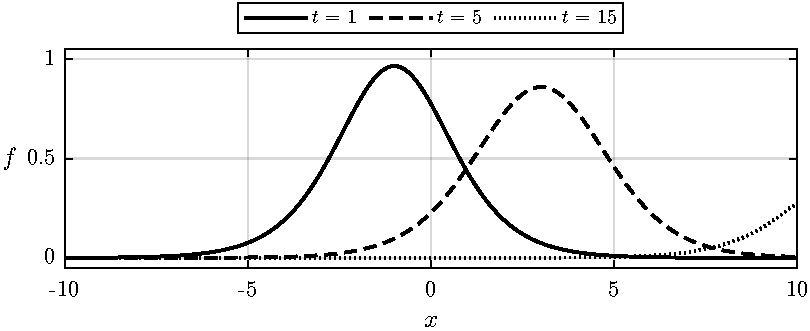
\includegraphics[width=0.85\linewidth]{fig_neumann.pdf}
\caption{Solution $f(x,t)$ of $\partial_t f + U\,\partial_x f = \alpha\,\partial_x^2 f$ with Neumann boundary conditions, $\partial_x f(\pm 10,t)=0$, at $t=1$, $5$ and $15$. Parameters: $U=1$, $\alpha=0.1$, $k=0.5$, $f(x,0)=\operatorname{sech}^2[k(x+2)]$. FTCS scheme with $N_x=201$ nodes ($\Delta x=0.1$) and $\Delta t=0.05$. All variables are dimensionless.}
\label{fig:neumann}
\end{figure}

\begin{figure}[H]
\centering
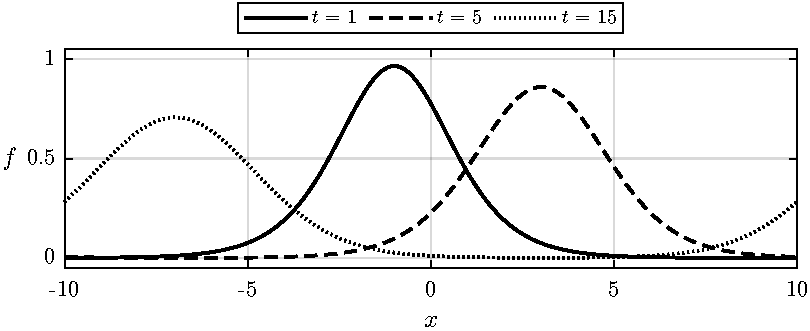
\includegraphics[width=0.85\linewidth]{fig_periodic.pdf}
\caption{Same equation and parameters as Fig.~\ref{fig:neumann} ($U=1$, $\alpha=0.1$, $k=0.5$, $N_x=201$, $\Delta t=0.05$) with periodic boundary conditions, $f(-10,t)=f(10,t)$, at $t=1$, $5$ and $15$. All variables are dimensionless.}
\label{fig:periodic}
\end{figure}

\small
\textbf{Dominant effect (assignment item 4).}
The pulse is displaced by $Ut$ while diffusion spreads it by only $\sqrt{2\alpha t}$. At $t=15$ in the figures, $Ut=15$ against $\sqrt{2\alpha t}\simeq1.7$, so advection dominates. The peak follows $x=-2+Ut$: $x\simeq-1$ and $3$ at $t=1,5$; in the periodic case it re-enters at $x\simeq-7$ ($13-20$), while with Neumann conditions it leaves through $x=10$ with zero slope. Runs at $t=5$ (periodic) confirm both limits. For $U\gg\alpha$ ($U=10$, $\alpha=0.1$) the pulse is transported without distortion ($\max f=0.99$, peak at $x\simeq 8$ as predicted). For $U\ll\alpha$ ($U=0.1$, $\alpha=10$) it barely moves ($Ut=0.5$) and diffuses to an almost flat profile ($\max f=0.20$, $\min f=0.20$). Stability needs, besides Eq.~(6), $\Delta t\le 2\alpha/U^2$ (effective diffusivity $\alpha-U^2\Delta t/2\ge0$), used here for $U\gg\alpha$.

\end{document}
